\subsection*{Problema 22}
\textbf{Enunciado:} Calcular la integral:
\begin{align*}
\int \dfrac{3x^2 + 3x + 1}{x^3 + 2x^2 + 2x + 1} \, dx
\end{align*}

\textbf{Solución:} 
Primero, factorizamos el denominador agrupando
términos o probando raíces racionales. 
Notamos que $x = -1$ es una raíz de 
$x^3 + 2x^2 + 2x + 1 = 0$. 
Dividiendo entre $x + 1$, obtenemos:
\begin{align*}
x^3 + 2x^2 + 2x + 1 = (x + 1)(x^2 + x + 1)
\end{align*}

Planteamos la descomposición en 
fracciones parciales según se indica:
\begin{align*}
\dfrac{3x^2 + 3x + 1}{(x + 1)(x^2 + x + 1)} = 
\dfrac{A}{x + 1} + \dfrac{Bx + C}{x^2 + x + 1}
\end{align*}

Multiplicando por el denominador común:
\begin{align*}
3x^2 + 3x + 1 &= A(x^2 + x + 1) \\
&\quad + (Bx + C)(x + 1)
\end{align*}

Expandimos y agrupamos términos por potencias de $x$:
\begin{align*}
3x^2 + 3x + 1 &= (A + B)x^2 \\
&\quad + (A + B + C)x + (A + C)
\end{align*}

Igualando los coeficientes de ambos lados:
\begin{align*}
A + B &= 3 \\
A + B + C &= 3 \\
A + C &= 1
\end{align*}

De la primera y segunda ecuación, 
sustituimos $A + B = 3$:
\begin{align*}
3 + C = 3 \implies C = 0
\end{align*}

Sustituyendo $C = 0$ en la tercera ecuación:
\begin{align*}
A + 0 = 1 \implies A = 1
\end{align*}

Y usando $A = 1$ en la primera ecuación:
\begin{align*}
1 + B = 3 \implies B = 2
\end{align*}

Sustituimos los valores de $A$, $B$ y $C$ 
en las fracciones parciales:
\begin{align*}
\int \left( \dfrac{1}{x + 1} + \dfrac{2x}{x^2 + x + 1} \right) dx
\end{align*}

Para la segunda integral, ajustamos el numerador 
para que sea la derivada del denominador 
($\dfrac{d}{dx}(x^2 + x + 1) = 2x + 1$):
\begin{align*}
\int \dfrac{2x}{x^2 + x + 1} dx &= \int \dfrac{2x + 1 - 1}{x^2 + x + 1} dx \\
&= \int \dfrac{2x + 1}{x^2 + x + 1} dx \\
&\quad - \int \dfrac{1}{(x + \frac{1}{2})^2 + \frac{3}{4}} dx
\end{align*}

Integramos cada término resultante:
\begin{align*}
\int \dfrac{1}{x + 1} dx &= \ln|x + 1| \\
\int \dfrac{2x + 1}{x^2 + x + 1} dx &= \ln|x^2 + x + 1| \\
\int \dfrac{1}{(x + \frac{1}{2})^2 + \frac{3}{4}} dx &= \dfrac{2}{\sqrt{3}} \arctan\left(\dfrac{2x + 1}{\sqrt{3}}\right)
\end{align*}

Juntando todas las antiderivadas, 
la solución general es:
\begin{align*}
F(x) &= \ln|x + 1| + \ln|x^2 + x + 1| \\
&\quad - \dfrac{2}{\sqrt{3}} \arctan\left(\dfrac{2x + 1}{\sqrt{3}}\right) + C
\end{align*}
O de forma compacta:
\begin{align*}
F(x) &= \ln|(x + 1)(x^2 + x + 1)| \\
&\quad - \dfrac{2}{\sqrt{3}} \arctan\left(\dfrac{2x + 1}{\sqrt{3}}\right) + C
\end{align*}

\begin{figure}[H]
	\centering
	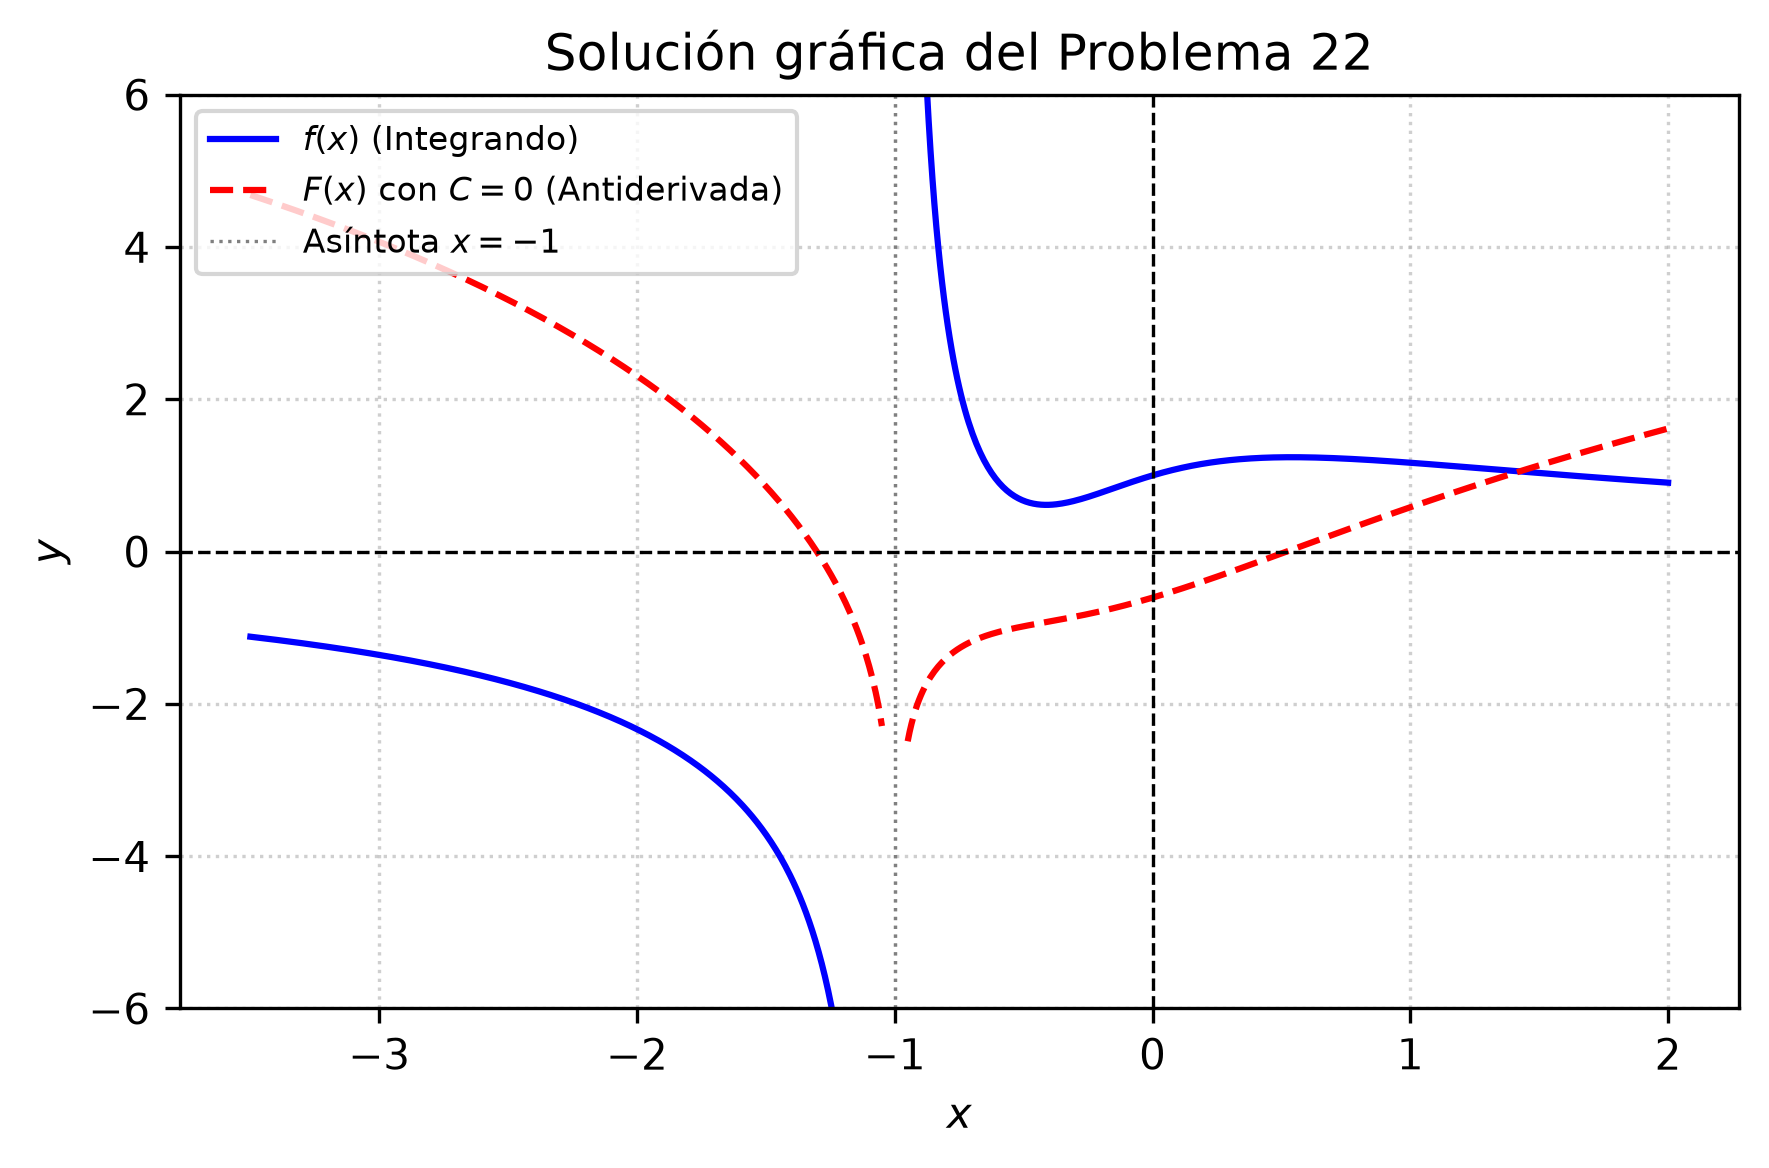
\includegraphics[width=\columnwidth]{semana_03/graficas/SEM03_P22_grafica.png}
	\caption{Representación gráfica de $f(x)$ y su antiderivada $F(x)$ evaluada para la constante de integración $C = 0$ (Problema 22).}
	\label{fig:problema22}
\end{figure}
